\documentclass[10pt, a4paper]{exam}
\usepackage{graphicx}
\usepackage[a4paper, total={7in, 9.5in}]{geometry}
\usepackage[normalem]{ulem}
\usepackage{amsmath}
\renewcommand\ULthickness{1.0pt}   
\setlength\ULdepth{1.3ex}

\begin{document}


	\noindent
	\begin{minipage}[l]{0.1\textwidth}
		\noindent
		
\includegraphics[width=2.8\textwidth]{ESCUDO.png}
	\end{minipage}
\hfill
\begin{minipage}[c]{0.8\textwidth}
	\begin{center}
		{\large  Departamento de Ingeniería civil y Agrícola\par
		\large	Facultad de Ingeniería	\par
	% \large \textbf{Taller propiedades de los fluidos}	\par
    \large \textbf{Banco de problemas\\Conceptos básicos - Flujo uniforme}	\par
} %%%%% NOMBRE DEL PROFESOR 
	\end{center}
\end{minipage}
\par
\vspace{0.2in}
\noindent
    \uline{Estructuras hidráulicas [2015954]	\hfill 2025-I}
\par 
\vspace{0.15in}
\noindent

%%%%%%%%%%%%%%%%%%%%%%%%%%%%%


En el presente taller se proponen un total de 25 ejercicios correspondientes a los temas \textit{Conceptos Básicos y Flujo Uniforme}, se tiene así:

\begin{enumerate}
    \item Un canal de sección trapezoidal (\(z = 1\)), base \(b = 2 \, \text{m}\), transporta un caudal \(Q = 4 \, \text{m}^3/\text{s}\) con una profundidad de flujo de \(y = 1.5 \, \text{m}\). Calcular los elementos geométricos e hidráulicos del flujo en la sección transversal. (Área de flujo, Perímetro mojado, Radio Hidráulico, Ancho superficial, Profundidad Hidráulica, Velocidad de flujo y número de froude).
 
    \item Se tiene un túnel con una sección transversal como se muestra en la Figura \ref{fig:tunredon}, calcular A, P, R  y T.

    \begin{figure}[h]
        \centering
        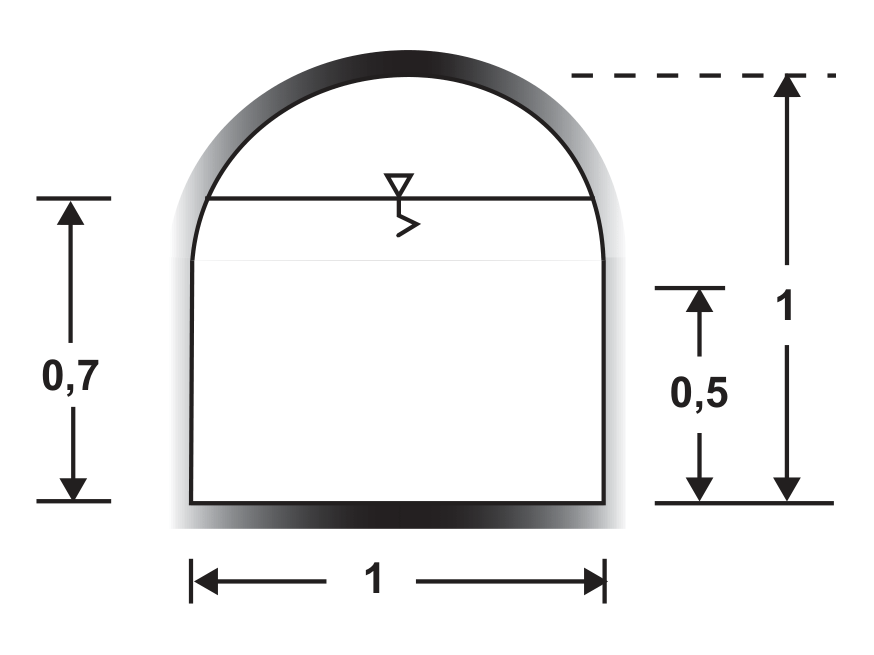
\includegraphics[width=0.32\linewidth]{Images/seccirc.png}
        \caption{Sección transversal del túnel, medidas en \textit{m}.}
        \label{fig:tunredon} 
    \end{figure}

    Para el segmento circular utilice:

    \begin{figure}[h]
        \centering
        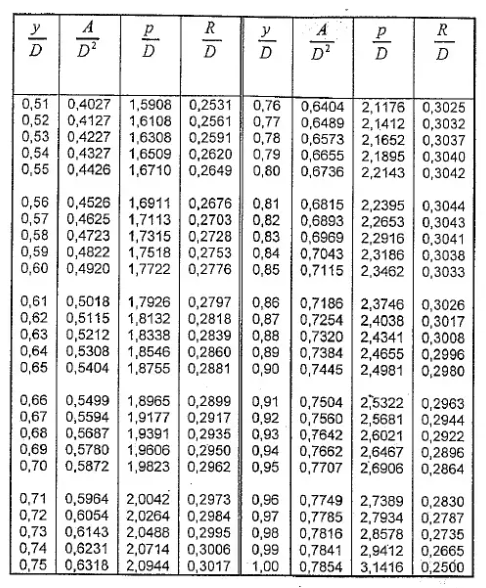
\includegraphics[width=0.4\linewidth]{Images/tabla.png}
        \caption{Área, perímetro mojado y radio hidráulico en conductos circulares parcialmente llenos.}
        \label{}
    \end{figure}

\newpage

    \item  Un canal de sección trapezoidal tiene una base de $0.80m$ y un talud $Z = 1$. En cierta sección de su perfil longitudinal, se construye una sobre-elevación de $0.15m$, pero se deja una abertura de $0.20m$ para evitar que el agua se empoce cuando se efectúa la limpieza del canal.

    Calcular $A$, $P$, $T$ y $R$ si la profundidad es de $0.90m$.

    
    \item Un canal de sección circular de $5m$ diámetro, conduce un caudal de $17 m^3/s$, con una velocidad de $1.5 m/s$. Indicar cuál es la profundidad.


    \item En un canal que conduce un caudal de $9 m^3/s$; existe una transición de salida, que sirve para unir una sección rectangular con una trapezoidal, cuyas dimensiones se muestran en la figura \ref{fig:trapezo}. Indicar cual es la velocidad en la sección rectangular. Considerar que las pérdidas en la sección 1 y 2 es solo por transición, siendo la fórmula para su cálculo:
    \begin{equation}
        h_{f1-2}=0.3\dfrac{v^2_1-v^2_2}{2g}
    \end{equation}

    \begin{figure}[h]
        \centering
        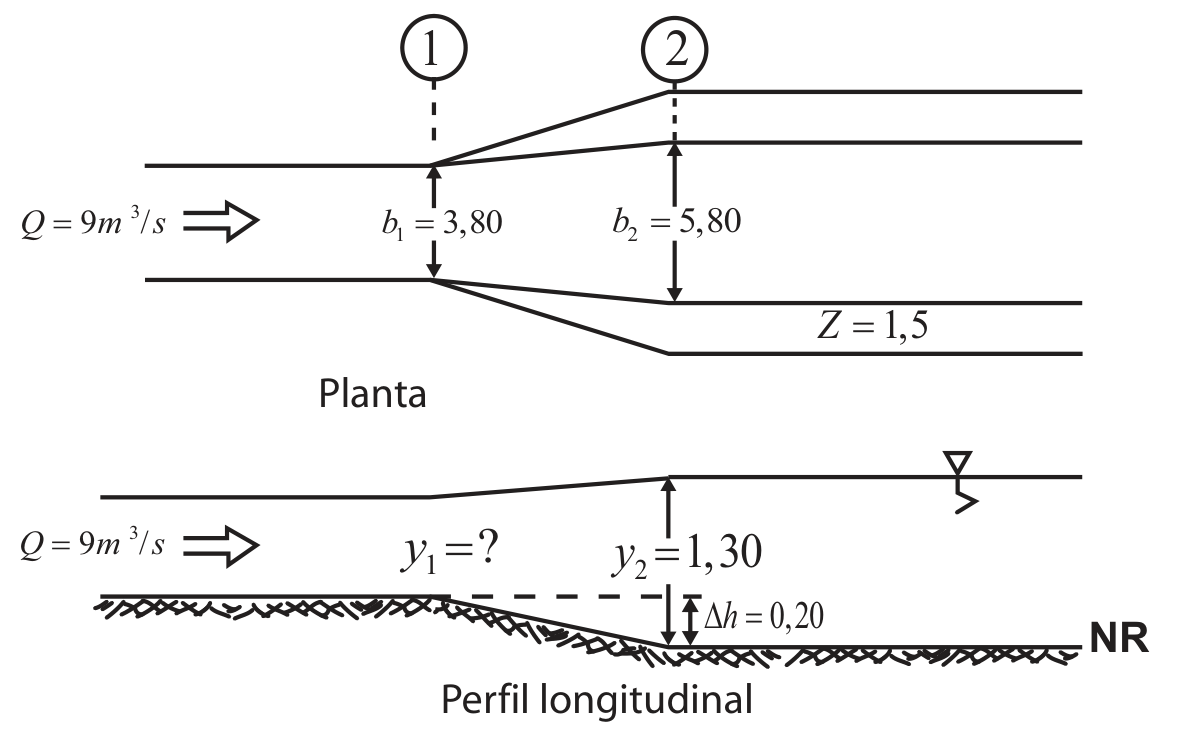
\includegraphics[width=0.6\linewidth]{Images/trapezo.png}
        \caption{Tramo de un canal.}
        \label{fig:trapezo}
    \end{figure}


    \item Para un canal trapecial con ancho de base $b = 6.0 m (20 ft)$ y talud o pendiente de $z=2$, calcúlese la profundidad crítica del flujo si $Q = 17 m^3/s (600 ft^3/s)$.

    \item Un vertedero de cresta ancha se coloca en un canal de ancho b (figura \ref{fig:ancho}). Si la profundidad del flujo aguas arriba es $y1$ y la carga de velocidad aguas arriba y las pérdidas por fricción pueden ser despreciadas, desarróllese una ecuación teórica para el caudal en términos del tirante del flujo aguas arriba.

    Tenga en cuenta que para un canal rectangular:

    \begin{equation}
        y_c=\left(\dfrac{q^2}{g}\right)^{1/3}  \quad  y_c=\dfrac{2}{3}E_c
    \end{equation}

    \begin{figure}[h]
        \centering
        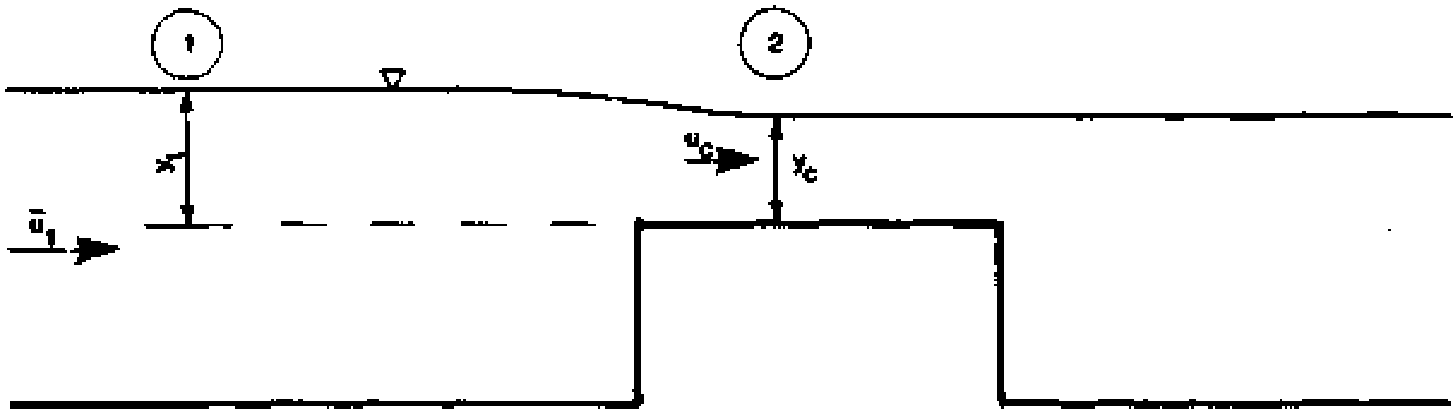
\includegraphics[width=0.6\linewidth]{Images/vertancho.png}
        \caption{Vertedero de cresta ancha.}
        \label{fig:ancho}
    \end{figure}

\newpage

    \item  Un canal rectangular se extiende suavemente desde un ancho de $1.5m (4.9 ft)$ a $3.0 m (9.8 ft)$. Aguas arriba de la expansión la profundidad del flujo es de $1.5 m (4.9 ft)$ y la velocidad del flujo es de $2.0 m/s (6.6 ft/s)$. Estímese el tirante del flujo después de la expansión.

    \item Considérese la sección transversal del colector representada en la figura \ref{fig:colector} La pendiente longitudinal de colector es 0.0004 y el coeficiente de Manning es 0.014. Determínese el caudal circulante (en régimen permanente y uniforme) para la profundidad máxima del flujo representada si el canal de caudales bajos es de geometría semicircular.

    \begin{figure}[h]
        \centering
        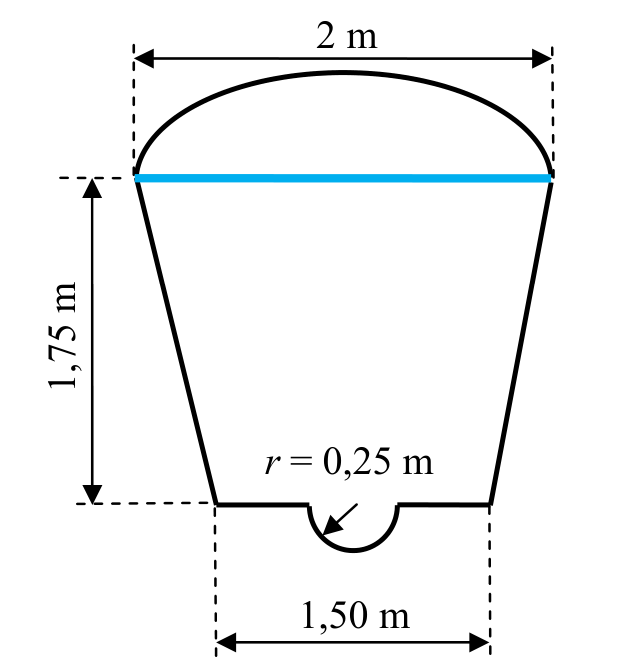
\includegraphics[width=0.3\linewidth]{Images/colector.png}
        \caption{Representación del colector.}
        \label{fig:colector}
    \end{figure}

    \item Calcúlese el caudal circulante en la sección del cauce de la figura \ref{fig:trapcompus} para flujo en régimen permanente y uniforme si la pendiente longitudinal es del 2\% y el coeficiente de Manning es igual a 0.045.

    \begin{figure}[h]
        \centering
        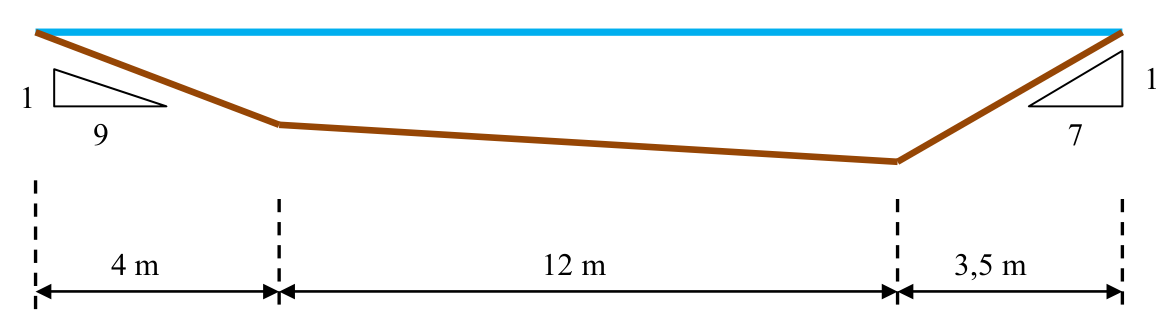
\includegraphics[width=0.6\linewidth]{Images/trapcompus.png}
        \caption{Sección del cause.}
        \label{fig:trapcompus}
    \end{figure}

    \item Sea un tramo de cauce de sección rectangular de $2m$ de anchura, pendiente longitudinal del 0.01\% y coeficiente de Manning de $0.015$. Determínese la profundidad del flujo en régimen permanente y uniforme si circula un caudal de $1m^3/s$.

    \item Determínese la profundidad crítica en una sección de geometría rectangular de $1m$ de ancho para un caudal de $1m^3/s$.

    \newpage

    \item Sea un canal de laboratorio de pendiente variable (entre el 0.001\% y el 2\%) cuya sección es triangular simétrica (véase la figura \ref{fig:triangulo}). Supóngase un tramo intermedio del canal en el que el flujo circula en régimen permanente y uniforme. Determínese el valor de la energía específica mínima en el canal para dicho tramo e intervalo de pendiente, si el caudal se mantiene constante a $0.4m^3/s$.

    \begin{figure}[h]
        \centering
        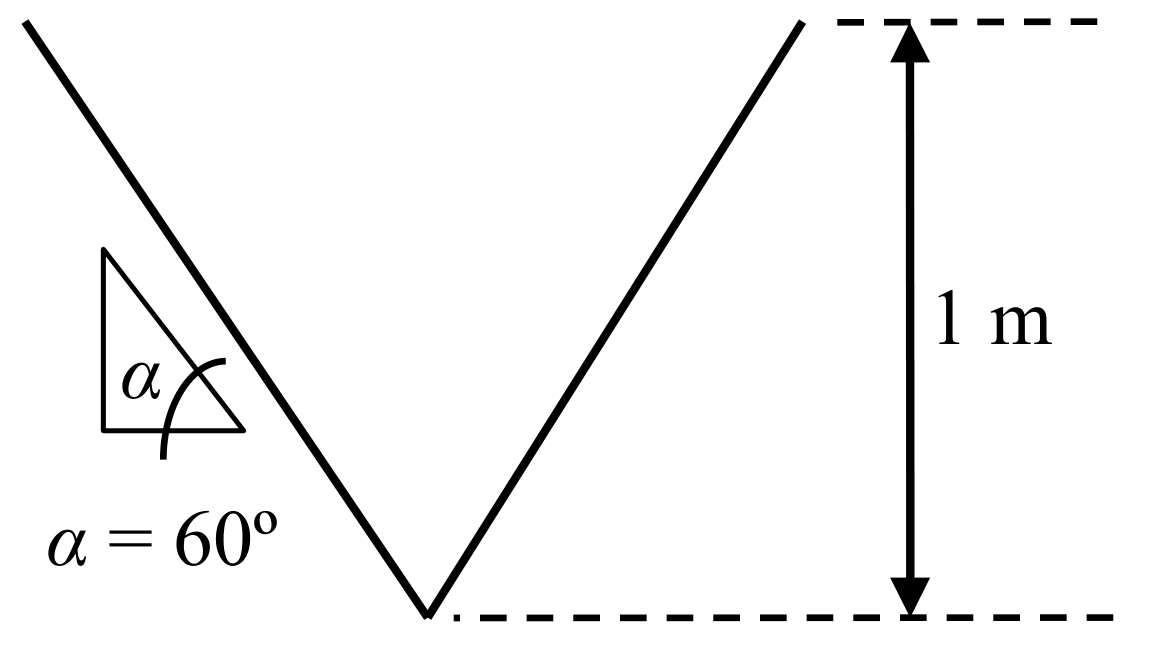
\includegraphics[width=0.35\linewidth]{Images/triang.png}
        \caption{Sección triangular.}
        \label{fig:triangulo}
    \end{figure}

    \item Calcúlese la profundidad crítica en la sección trapecial de la figura \ref{traparbo} adjunta si el caudal circulante es de $45m^3/s$.

    \begin{figure}[h]
        \centering
        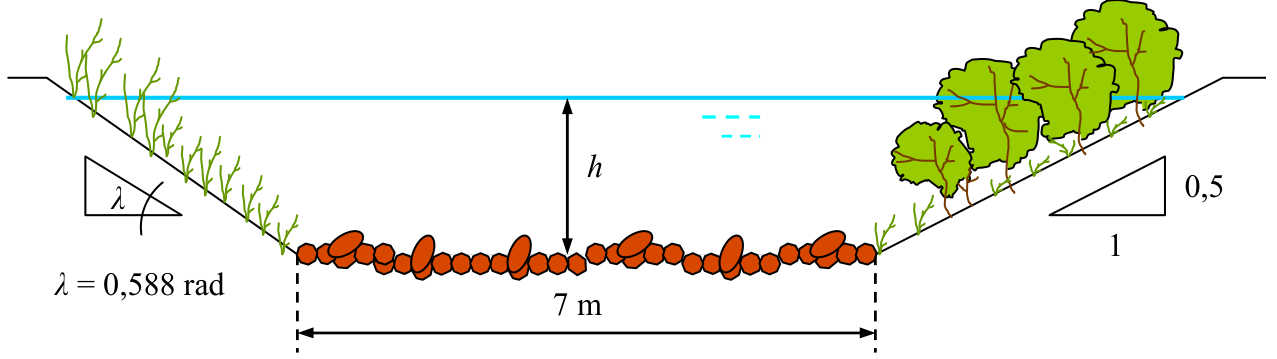
\includegraphics[width=0.7\linewidth]{Images/traparbo.png}
        \caption{Sección trapezoidal.}
        \label{traparbo}
    \end{figure}

    \item Un depósito alimenta a un canal trapezoidal de ancho de $1m$, talud $Z=1$, coeficiente de rugosidad $0.014$ y pendiente $0.0005$. A la entrada, la profundidad de agua en el depósito es de $0.736 m$ por encima del fondo del canal como se muestra en la figura \ref{deposit}. Determinar el caudal en el canal con flujo uniforme subcrítico, suponiendo que la pérdida a la entrada es $0.25 \cdot v^2_1/2g$.

    \begin{figure}[h]
        \centering
        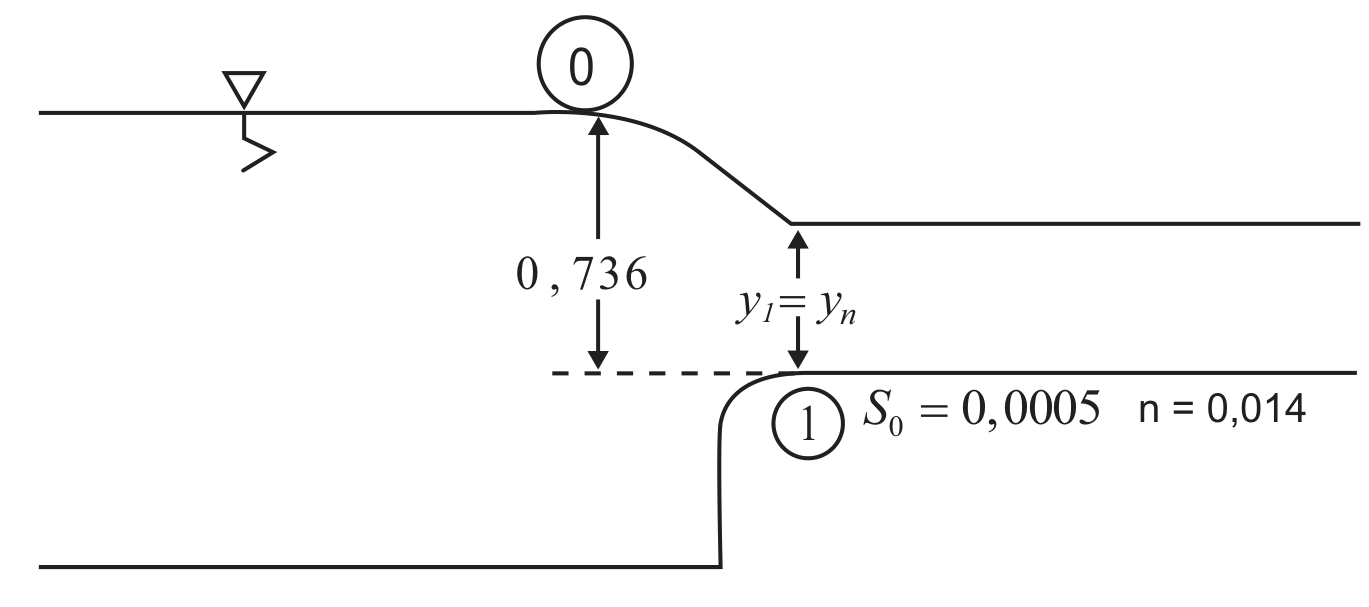
\includegraphics[width=0.5\linewidth]{Images/deposit.png}
        \caption{Perfil longitudinal del depósito y canal.}
        \label{deposit}
    \end{figure}    

    \item Dado un canal tropical con un ancho en el fondo de $3m (10 ft)$, con taludes $1.5:1$, una pendiente longitudinal de $0.0016$, y un coeficiente de manning $n = 0.013$, determínese el caudal si la profundidad normal del flujo es de $ 2.6 m (8.5 ft)$.

    \item Por un canal trapezoidal de pendiente de paredes 3 vertical y 2 horizontal (talud $Z = \frac{3}{2}$), con un ancho de $0.8m$, circula agua con una velocidad en $m/s$, numéricamente igual al ancho. Determinar el caudal que lleva el canal si el coeficiente de rugosidad es $0.025$ y la pendiente 0.3\%.

    \newpage

    \item Water flows in a rectangular, concrete, open channel that is $12 m$ wide at a depth of $2.5m$. The channel slope is $0.0028$. Find the water velocity and the flow rate. $(n = 0.013)$ 

    \item Water flows in a rectangular, concrete, open channel that is $12 m$ wide. The channel slope is $0.0028$. If the velocity of the flow is $6 m/s$, find the depth of the flow. $(n = 0.013)$ 

    \begin{figure}[h]
        \centering
        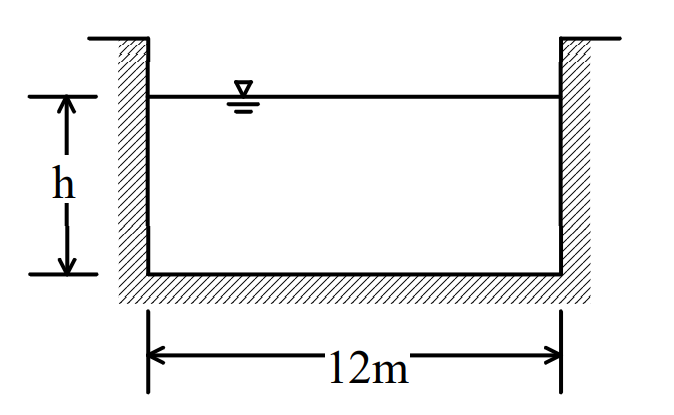
\includegraphics[width=0.3\linewidth]{Images/recfinal.png}
        \caption{Canal revestido de concreto.}
        \label{}
    \end{figure} 

    \item A trapezoidal channel with side slopes of 2/3, a depth of $2 m$, a bottom width of $8 m$ and a channel slope of $0.0009$ has a discharge of $56 m^3/s$. Find the Manning’s n. 

    \begin{figure}[h]
        \centering
        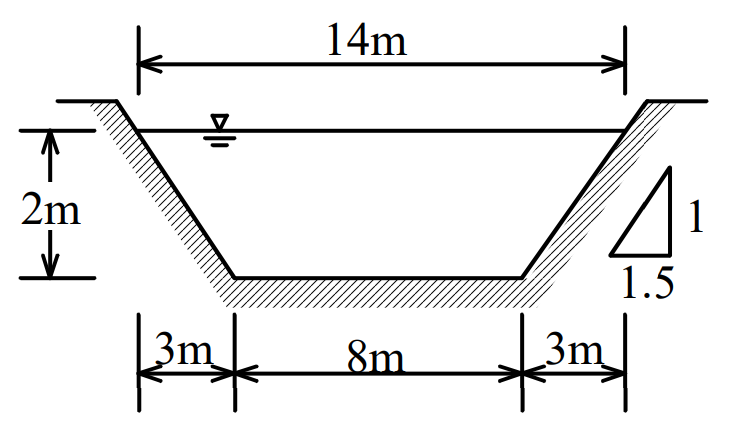
\includegraphics[width=0.3\linewidth]{Images/trapfinal.png}
        \caption{Canal trapezoidal.}
        \label{}
    \end{figure} 

    \item Determine the depth in a trapezoidal channel with side slopes of 1 to 1.5, a bottom width of $8 m$ and a channel slope of $0.0009$. The discharge is $56 m^3/s$ and $n=0.017$.

    \begin{figure}[h]
        \centering
        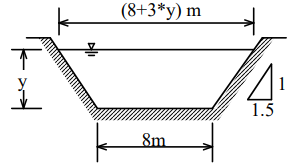
\includegraphics[width=0.3\linewidth]{Images/trapfinal2.png}
        \caption{Canal trapezoidal.}
        \label{}
    \end{figure} 

    \item Water flows at a depth of $2.20 m$ in a trapezoidal, concrete-lined section $(ks = 2 mm)$ with a bottom width of $3.6 m$ and side slopes of $2:1 (H:V)$. The slope of the channel is $0.0006$ and the water temperature is $20^\circ C$. Assuming uniform-flow conditions, estimate the average velocity and flowrate in the channel. Use both the Darcy-Weisbach and Manning equations and compare your answers.

    \item Determine the critical depth for $30 m^3/s$ flowing in a rectangular channel with width $5 m$. If the depth of flow is equal to $3 m$, is the flow supercritical or subcritical?

    \item A rectangular channel $2 m$ wide carries $3 m^3/s$ of water at a depth of $1.2 m$. If an obstruction $40 cm$ wide is placed in the middle of this channel, find the elevation of the water surface at the constriction. What is the minimum width of the constriction that will not cause a rise in the water surface upstream?

    \item Water flows at $4.3 m^3/s$ in a rectangular channel of width $3 m$ and depth of flow $1 m$. If the channel width is decreased by $0.75 m$ and the bottom of the channel is raised by $0.25 m$, what is the depth of flow in the constriction?
    


\end{enumerate}

    
\end{document}



